\documentclass[aspectratio=169,11pt]{beamer}

\usepackage[utf8]{inputenc}
\usepackage[T1]{fontenc}
\usepackage{graphicx}
\usepackage{array}
\usepackage{tabularx}
\usepackage{xcolor}

\usetheme{Madrid}
\usecolortheme{default}
\setbeamertemplate{navigation symbols}{}
\setbeamertemplate{footline}[frame number]

\definecolor{spityGreen}{HTML}{1F8A5B}
\definecolor{spityDark}{HTML}{17231F}
\definecolor{spitySand}{HTML}{F4EFE6}
\definecolor{spityOrange}{HTML}{D97706}
\definecolor{spityRed}{HTML}{B42318}

\setbeamercolor{title}{fg=white,bg=spityDark}
\setbeamercolor{frametitle}{fg=white,bg=spityDark}
\setbeamercolor{structure}{fg=spityGreen}
\setbeamercolor{block title}{fg=white,bg=spityGreen}
\setbeamercolor{block body}{bg=spitySand!45}

\newcommand{\competence}[2]{%
  \begin{block}{#1}
    #2
  \end{block}
}

\title[Spity -- Bloc 01]{Spity}
\subtitle{Cadrer un projet de développement d'application logicielle\\Bloc 01 -- RNCP 39583}
\author{Dorian Joly}
\institute{Expert en développement logiciel}
\date{Soutenance RNCP}

\begin{document}

\begin{frame}
  \titlepage
  \vspace{-0.5cm}
  \begin{center}
    
\includegraphics[height=1.2cm]{../../../spity/public/images/brand/logo-spity.png}
  \end{center}
\end{frame}

\begin{frame}{Objectif de la présentation}
  \begin{columns}[T]
    \begin{column}{0.54\textwidth}
      \begin{block}{But}
        Démontrer que le projet Spity est cadré, faisable, priorisé et défendable devant un commanditaire.
      \end{block}
      \begin{itemize}
        \item Présenter le besoin métier et la problématique.
        \item Montrer les preuves attendues par la grille Bloc 01.
        \item Justifier les choix techniques, budgétaires et de sécurité.
        \item Obtenir une validation de lancement MVP.
      \end{itemize}
    \end{column}
    \begin{column}{0.42\textwidth}
      \begin{block}{Fil directeur}
        \begin{enumerate}
          \item Contexte et acteurs
          \item Analyse et faisabilité
          \item Veille et architecture
          \item Charge, coût et risques
          \item Préconisation finale
        \end{enumerate}
      \end{block}
    \end{column}
  \end{columns}
\end{frame}

\begin{frame}[shrink=6]{Lecture de la grille d'évaluation}
  \small
  \begin{tabularx}{\textwidth}{>{\bfseries}p{1.8cm} X X}
    Comp. & Attendu jury & Preuve présentée \\
    \hline
    C1.1.1 & Cartographie des acteurs et futurs utilisateurs & RACI, personas, niveaux d'implication \\
    C1.1.2 & Analyse de la demande, objectifs et enjeux & Problématique, attentes, pistes de solution \\
    C1.2.1 & Opportunités, menaces, environnement, sécurité & SWOT et points de vigilance \\
    C1.2.2 & Faisabilité technique et diagnostic & Audit stack, contraintes, avis de lancement \\
    C1.2.3 & Risques et indicateurs de contrôle & Matrice risques, criticité, KPI de suivi \\
    C1.3.1 & Veille technique, réglementaire, environnementale & Sources, méthode, impacts métier \\
    C1.3.2 & Comparatif d'architectures & Options comparées et choix argumenté \\
    C1.4.1 & Fonctions et charge en jour-homme & Lots MVP, priorisation, estimation \\
    C1.4.2 & Budget prévisionnel & Coûts développement, infra, services \\
    C1.5 & Architecture logicielle modélisée & Schéma applicatif et choix de formalisme \\
    C1.6 & Préconisation argumentée & Décision proposée et traitement objections \\
  \end{tabularx}
\end{frame}

\section{Projet}

\begin{frame}{Spity en une phrase}
  \begin{columns}[T]
    \begin{column}{0.48\textwidth}
      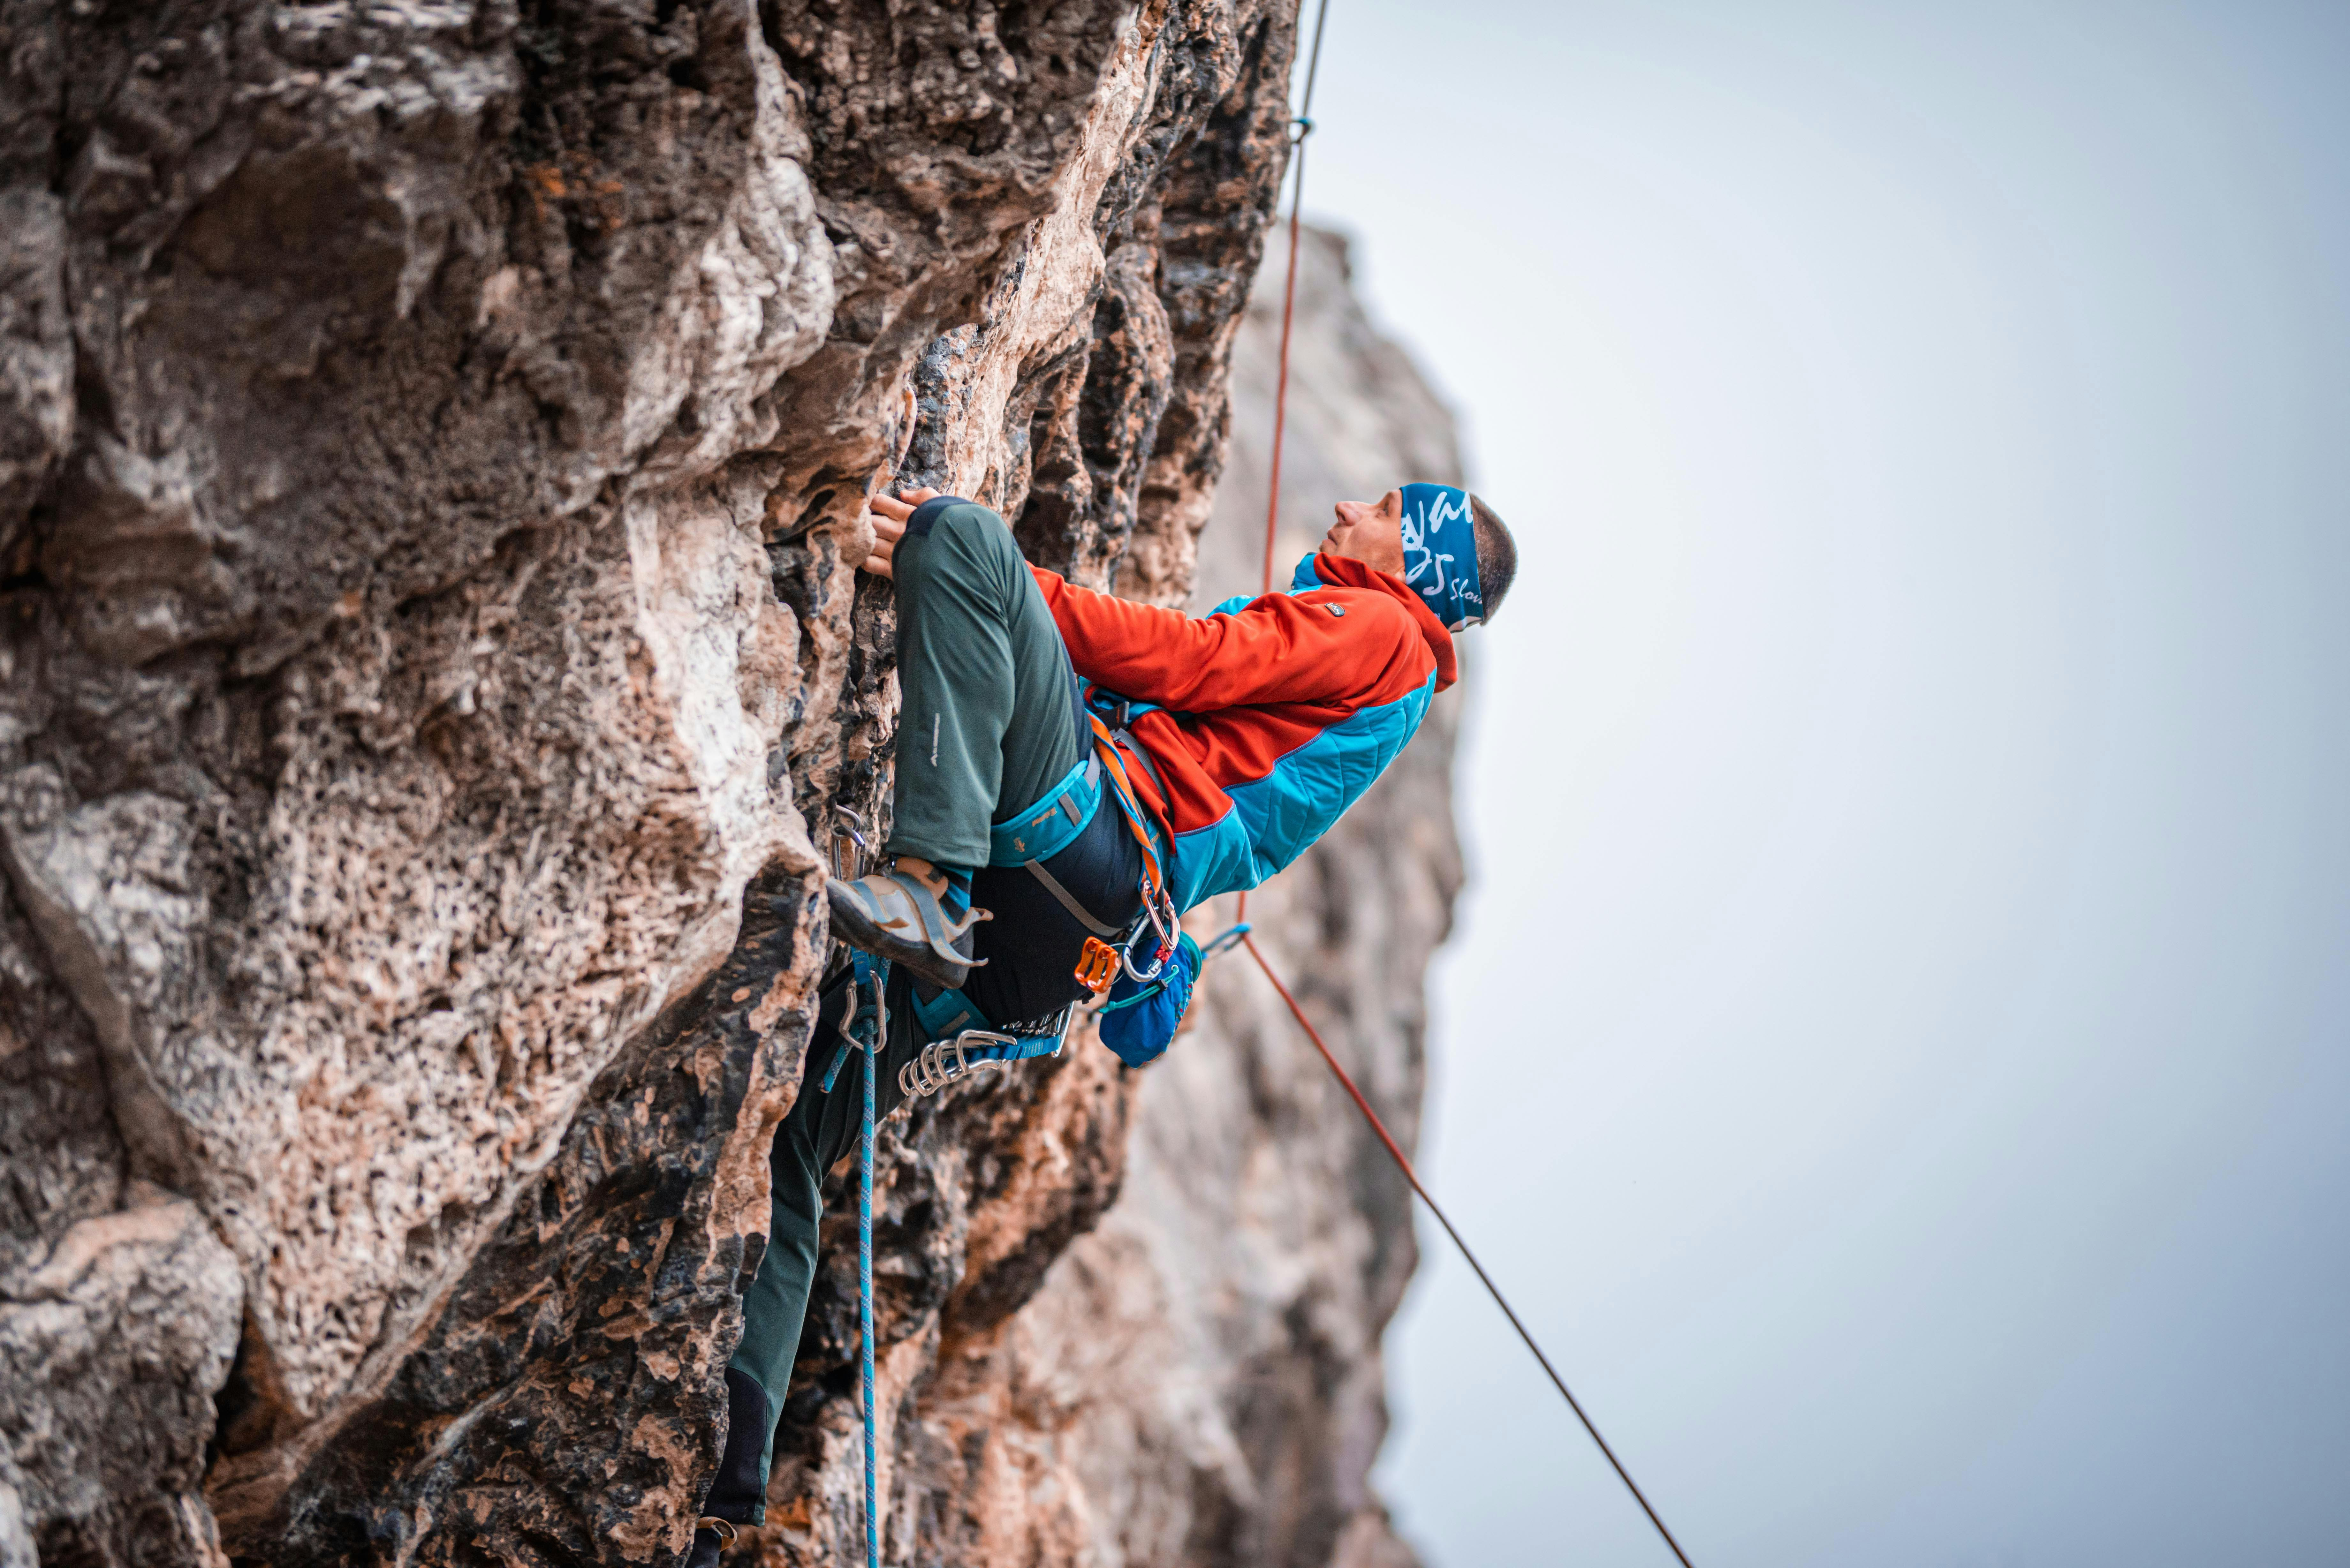
\includegraphics[width=\textwidth,height=0.55\textheight,keepaspectratio]{../../../spity/public/images/brand/escalade-falaise.jpeg}
    \end{column}
    \begin{column}{0.48\textwidth}
      \begin{block}{Vision}
        Spity est un réseau social complet pour la communauté escalade : matching de grimpeurs, topos collaboratifs, répertoire de salles/falaises/clubs et événements.
      \end{block}
      \begin{itemize}
        \item Projet support de certification RNCP.
        \item MVP démontrable pour la soutenance.
        \item Zone pilote : Lyon, Grenoble, Rhône-Alpes.
      \end{itemize}
    \end{column}
  \end{columns}
\end{frame}

\begin{frame}{Contexte marché}
  \begin{columns}[T]
    \begin{column}{0.5\textwidth}
      \begin{block}{Constat}
        L'escalade progresse fortement, mais l'information reste éclatée entre groupes sociaux, sites de salles, clubs, topos papier et applications spécialisées.
      \end{block}
      \begin{itemize}
        \item Plus de 300 000 licenciés FFME.
        \item Plus de 1 200 clubs affiliés.
        \item Plus de 800 salles indoor.
        \item Besoin fort de données locales et à jour.
      \end{itemize}
    \end{column}
    \begin{column}{0.46\textwidth}
      \begin{block}{Opportunité}
        Unifier les usages quotidiens des grimpeurs dans une plateforme sociale contextualisée.
      \end{block}
      \begin{itemize}
        \item Trouver un partenaire compatible.
        \item Identifier les lieux et événements proches.
        \item Partager des performances avec contexte technique.
        \item Signaler les informations sécurité terrain.
      \end{itemize}
    \end{column}
  \end{columns}
\end{frame}

\begin{frame}{Problématique client}
  \begin{block}{Problème principal}
    Les grimpeurs jonglent entre plusieurs sources pour une seule activité, perdent du temps et manquent d'informations fiables, locales et actualisées.
  \end{block}
  \vspace{0.2cm}
  \begin{tabularx}{\textwidth}{>{\bfseries}p{3.2cm} X X}
    Besoin & Solution actuelle & Limite identifiée \\
    \hline
    Partenaires & Groupes Facebook & Peu de filtrage, confiance faible \\
    Topos & Papier, Camptocamp & Données statiques, sécurité peu temps réel \\
    Clubs & Sites et réseaux séparés & Visibilité faible, événements dispersés \\
    Salles & Sites disparates & Infos parfois obsolètes, pas de lien social \\
    Partage social & Instagram & Pas de cotation, lieu, matériel ou discipline \\
  \end{tabularx}
\end{frame}

\section{C1.1 -- Acteurs et demande}

\begin{frame}{C1.1.1 -- Parties prenantes}
  \competence{Livrable attendu}{Cartographie des parties prenantes avec rôles, niveau d'implication et futurs utilisateurs.}
  \small
  \begin{tabularx}{\textwidth}{>{\bfseries}p{2.6cm} p{2.1cm} X p{2.2cm}}
    Acteur & Rôle & Contribution au MVP & Implication \\
    \hline
    Grimpeurs & Utilisateurs finaux & Profil, posts, matching, votes topos & Très forte \\
    Clubs FFME & Partenaires actifs & Création d'événements, coachs, validation club & Forte \\
    Salles & Partenaires passifs puis actifs & Fiches lieux, horaires, offres & Moyenne \\
    Équipeurs & Experts terrain & Signalements, sécurité, cotations & Moyenne \\
    Développeur & Réalisation & Cadrage, architecture, développement, démo & Forte \\
    FFME & Institution & Référentiel, visibilité, perspective V2 & Faible en MVP \\
  \end{tabularx}
\end{frame}

\begin{frame}{Futurs utilisateurs ciblés}
  \begin{columns}[T]
    \begin{column}{0.32\textwidth}
      \begin{block}{Grimpeur urbain}
        \small
        25--45 ans, pratique salle en semaine et falaise le week-end. Cherche partenaires fiables, événements locaux et suivi de progression.
      \end{block}
    \end{column}
    \begin{column}{0.32\textwidth}
      \begin{block}{Club local}
        \small
        Souhaite gagner en visibilité, centraliser les inscriptions et communiquer simplement sur les sorties, initiations et coachings.
      \end{block}
    \end{column}
    \begin{column}{0.32\textwidth}
      \begin{block}{Contributeur falaise}
        \small
        Partage l'état des voies, photos, cotations et alertes sécurité pour maintenir des topos vivants et utiles.
      \end{block}
    \end{column}
  \end{columns}
  \vspace{0.3cm}
  \begin{block}{Critère couvert}
    Les caractéristiques des futurs utilisateurs sont identifiées, détaillées et reliées aux fonctionnalités MVP.
  \end{block}
\end{frame}

\begin{frame}{C1.1.2 -- Analyse de la demande}
  \competence{Livrable attendu}{Présentation de l'analyse de la demande, des objectifs et des enjeux pour chaque partie prenante.}
  \begin{columns}[T]
    \begin{column}{0.48\textwidth}
      \begin{block}{Objectifs métier}
        \begin{itemize}
          \item Réduire la fragmentation des usages escalade.
          \item Fiabiliser les informations de lieux et de sécurité.
          \item Créer une base d'utilisateurs suffisante pour un feed vivant.
          \item Faciliter l'activité des clubs locaux.
        \end{itemize}
      \end{block}
    \end{column}
    \begin{column}{0.48\textwidth}
      \begin{block}{Pistes de solution}
        \begin{itemize}
          \item Profils grimpeur et club.
          \item Fil social contextualisé.
          \item Répertoire géolocalisé.
          \item Topos collaboratifs.
          \item Calendrier club avec inscriptions.
        \end{itemize}
      \end{block}
    \end{column}
  \end{columns}
\end{frame}

\section{C1.2 -- Opportunités, faisabilité, risques}

\begin{frame}{C1.2.1 -- Opportunités et menaces}
  \competence{Livrable attendu}{Cartographie opportunités/menaces, impact environnemental, sécurité et points de vigilance.}
  \small
  \begin{tabularx}{\textwidth}{>{\bfseries}p{2.4cm} X X}
    Axe & Opportunités à exploiter & Menaces à contrôler \\
    \hline
    Marché & Croissance escalade, clubs en recherche de visibilité & Concurrence plateformes sociales généralistes \\
    Usage & Données locales, matching, social contextualisé & Effet réseau lent au démarrage \\
    Sécurité & Alertes équipement, accès, état des voies & Responsabilité sur données terrain erronées \\
    Environnement & Mutualiser informations, limiter déplacements inutiles & Stockage médias et trafic cartographique \\
    Technique & Stack web unifiée, déploiement rapide & Dette technique si MVP trop large \\
  \end{tabularx}
\end{frame}

\begin{frame}{Actions de maîtrise issues de la cartographie}
  \begin{columns}[T]
    \begin{column}{0.48\textwidth}
      \begin{block}{Sécurité et RGPD}
        \begin{itemize}
          \item Validation Zod des entrées API.
          \item Sessions sécurisées et protection CSRF.
          \item Rate limiting sur auth et uploads.
          \item Export/suppression compte à prévoir.
        \end{itemize}
      \end{block}
    \end{column}
    \begin{column}{0.48\textwidth}
      \begin{block}{Impact environnemental}
        \begin{itemize}
          \item Images compressées et stockées via CDN.
          \item Pagination et chargement progressif.
          \item Données géolocalisées filtrées par rayon.
          \item Hébergement dimensionné au MVP.
        \end{itemize}
      \end{block}
    \end{column}
  \end{columns}
\end{frame}

\begin{frame}[shrink=6]{C1.2.2 -- Faisabilité technique}
  \competence{Livrable attendu}{Démarche d'audit, diagnostic de l'existant, contraintes et avis critique sur la faisabilité.}
  \small
  \begin{tabularx}{\textwidth}{>{\bfseries}p{3.1cm} X X}
    Domaine audité & Diagnostic & Décision MVP \\
    \hline
    Frontend & Besoin d'interface riche, mobile-first, accessible & Next.js App Router, Tailwind, composants UI \\
    Backend & API web, auth, profils, contenus, lieux & Route Handlers Next.js, Zod, services métier \\
    Données & Relations utilisateurs, posts, lieux, événements & MariaDB + Drizzle ORM \\
    Médias & Photos/vidéos posts, lieux, topos & Cloudinary ou S3 en V1 \\
    Cartographie & Recherche par distance et pins & Leaflet ou Mapbox selon budget/API \\
    Qualité & Jury technique, sécurité, maintenabilité & ESLint, typecheck, tests ciblés \\
  \end{tabularx}
  \vspace{0.2cm}
  \begin{block}{Avis de faisabilité}
    Faisable en MVP si le périmètre reste centré sur profils, feed, lieux, topos et événements, avec priorisation stricte.
  \end{block}
\end{frame}

\begin{frame}{Contraintes identifiées}
  \begin{columns}[T]
    \begin{column}{0.5\textwidth}
      \begin{block}{Contraintes projet}
        \begin{itemize}
          \item Délais de soutenance courts.
          \item Démonstration attendue, pas seulement maquette.
          \item Données de démo crédibles.
          \item Budget limité pour services externes.
        \end{itemize}
      \end{block}
    \end{column}
    \begin{column}{0.46\textwidth}
      \begin{block}{Contraintes techniques}
        \begin{itemize}
          \item Authentification et données personnelles.
          \item Upload média et modération.
          \item Données de localisation.
          \item Accessibilité RGAA sur parcours critiques.
        \end{itemize}
      \end{block}
    \end{column}
  \end{columns}
\end{frame}

\begin{frame}{C1.2.3 -- Cartographie des risques}
  \competence{Livrable attendu}{Référentiel risques techniques et fonctionnels, priorisation, indicateurs de contrôle.}
  \tiny
  \begin{tabularx}{\textwidth}{>{\bfseries}p{1.2cm} p{2.8cm} p{1.6cm} X X}
    ID & Risque & Criticité & Mesure de maîtrise & Indicateur \\
    \hline
    R1 & Perte ou corruption de données & Élevée & ORM, migrations, sauvegardes, tests repository & Taux erreurs DB, restauration testée \\
    R2 & Interruption service & Moyenne & Déploiement simple, healthcheck, logs & Disponibilité, temps de réponse \\
    R3 & Données sécurité falaise erronées & Élevée & Modération, source, date, statut, signalement & Alertes ouvertes, délai traitement \\
    R4 & Fuite données personnelles & Élevée & Hash mot de passe, sessions sûres, RGPD, moindre privilège & Incidents sécurité, audit endpoints \\
    R5 & Périmètre MVP trop large & Élevée & MoSCoW, backlog, lots démo & Écart charge réelle/estimée \\
    R6 & Faible adoption initiale & Moyenne & Zone pilote, clubs partenaires, données demo & Inscrits, D7, posts/jour \\
  \end{tabularx}
\end{frame}

\section{C1.3 -- Veille et architecture}

\begin{frame}{C1.3.1 -- Veille technique et réglementaire}
  \competence{Livrable attendu}{Méthode de veille, sources consultées, outils, bénéfices et classification des évolutions.}
  \begin{columns}[T]
    \begin{column}{0.48\textwidth}
      \begin{block}{Méthode}
        \begin{itemize}
          \item Veille hebdomadaire ciblée.
          \item Sources officielles et documentation éditeur.
          \item Comparaison sécurité, coût, maintenabilité.
          \item Synthèse par impact métier/environnemental.
        \end{itemize}
      \end{block}
    \end{column}
    \begin{column}{0.48\textwidth}
      \begin{block}{Axes suivis}
        \begin{itemize}
          \item Next.js, React, Drizzle, MariaDB.
          \item OWASP Top 10, RGPD, cookies.
          \item RGAA et accessibilité clavier.
          \item Optimisation images, CDN, sobriété.
        \end{itemize}
      \end{block}
    \end{column}
  \end{columns}
\end{frame}

\begin{frame}{Apports de la veille au projet}
  \small
  \begin{tabularx}{\textwidth}{>{\bfseries}p{3cm} X X}
    Sujet & Décision prise & Impact \\
    \hline
    App Router & Utiliser les Route Handlers et Server Components lorsque pertinent & Moins de code client, meilleure maintenabilité \\
    Zod & Valider systématiquement entrées et sorties API & Réduction des erreurs et risques d'injection \\
    Drizzle & Typage fort du schéma et migrations versionnées & Traçabilité et sécurité des évolutions DB \\
    RGPD & Prévoir consentement, export et suppression compte & Conformité et confiance utilisateur \\
    RGAA & Composants accessibles clavier et contrastes AA & Parcours critiques utilisables par tous \\
    Images & Compression, formats adaptés, CDN & Performance et impact environnemental maîtrisé \\
  \end{tabularx}
\end{frame}

\begin{frame}{C1.3.2 -- Comparatif des architectures}
  \competence{Livrable attendu}{Étude comparative des solutions techniques, sécurité, systèmes, réseau, accessibilité, environnement.}
  \tiny
  \begin{tabularx}{\textwidth}{>{\bfseries}p{2.5cm} X X X}
    Option & Avantages & Limites & Verdict \\
    \hline
    No-code + SaaS & Rapide, faible coût initial & Verrouillage fournisseur, sécurité et modèle métier limités & Écarté \\
    Next.js monolithe modulaire & Front/API unifiés, typage, déploiement simple, bon MVP & Discipline nécessaire pour éviter couplage excessif & Retenu \\
    Microservices + mobile natif & Très scalable, séparation forte & Trop coûteux, trop complexe pour soutenance MVP & V2 possible \\
    Headless CMS + custom app & Back-office rapide & Logique sociale/matching/topos moins adaptée & Écarté \\
  \end{tabularx}
  \vspace{0.2cm}
  \begin{block}{Choix retenu}
    Architecture web modulaire Next.js + MariaDB + Drizzle, avec séparation par features et services externes limités au besoin.
  \end{block}
\end{frame}

\begin{frame}{C1.5 -- Architecture logicielle proposée}
  \competence{Livrable attendu}{Schéma légendé, formalisme justifié, interactions systèmes, sécurité, maintenabilité, extensibilité.}
  \small
  \begin{center}
    \begin{tabular}{c}
      Utilisateur web/mobile \\
      $\downarrow$ HTTPS \\
      Next.js App Router \\
      $\downarrow$ Server Components / Route Handlers \\
      Services métier par feature \\
      $\downarrow$ Drizzle ORM \\
      MariaDB \\
    \end{tabular}
  \end{center}
  \begin{columns}[T]
    \begin{column}{0.48\textwidth}
      \begin{block}{Services externes}
        Cloudinary/S3 pour médias, Leaflet/Mapbox pour carte, email pour OTP/notifications.
      \end{block}
    \end{column}
    \begin{column}{0.48\textwidth}
      \begin{block}{Formalisme}
        Architecture en couches et découpage feature-based, adapté à un MVP maintenable et évolutif.
      \end{block}
    \end{column}
  \end{columns}
\end{frame}

\begin{frame}{Qualités de l'architecture}
  \begin{columns}[T]
    \begin{column}{0.32\textwidth}
      \begin{block}{Maintenable}
        \small
        Features séparées, composants UI réutilisables, schémas Zod colocalisés, accès DB centralisé.
      \end{block}
    \end{column}
    \begin{column}{0.32\textwidth}
      \begin{block}{Sécurisée}
        \small
        Validation serveur, hash des mots de passe, cookies httpOnly, contrôle des rôles club/admin.
      \end{block}
    \end{column}
    \begin{column}{0.32\textwidth}
      \begin{block}{Extensible}
        \small
        Ajout possible d'app mobile, recommandations avancées, partenariat FFME et notifications push.
      \end{block}
    \end{column}
  \end{columns}
  \vspace{0.3cm}
  \begin{block}{Sobriété}
    Rendu serveur quand utile, chargement progressif, limitation des données cartographiques et médias optimisés.
  \end{block}
\end{frame}

\section{C1.4 -- Charge et budget}

\begin{frame}{C1.4.1 -- Fonctionnalités MVP hiérarchisées}
  \competence{Livrable attendu}{Fonctions recensées, caractérisées, ordonnées, charge en jour-homme et prise en compte UX.}
  \small
  \begin{tabularx}{\textwidth}{>{\bfseries}p{2.6cm} p{2cm} X}
    Lot & Priorité & Fonctionnalités \\
    \hline
    Authentification & Must & Inscription, connexion, session, protection routes \\
    Profils & Must & Grimpeur, club, niveaux, disciplines, matériel \\
    Feed social & Must & Posts contextualisés, likes, commentaires simples \\
    Répertoire & Must & Salles, falaises, clubs, recherche, filtres \\
    Topos & Should & Voies, cotations, statut, signalements \\
    Événements & Should & Création club, inscription, capacité \\
    Matching & Could & Recommandation simple par niveau/discipline/distance \\
    Notifications & Could & Push/email pour événements proches \\
  \end{tabularx}
\end{frame}

\begin{frame}{Estimation de charge}
  \small
  \begin{tabularx}{\textwidth}{>{\bfseries}p{3.2cm} p{2cm} X}
    Lot & Charge & Hypothèse \\
    \hline
    Cadrage, UX, backlog & 8 j.h & Ateliers, wireframes, priorisation \\
    Setup technique & 6 j.h & Next.js, Docker, DB, CI minimale \\
    Auth et sécurité de base & 10 j.h & Auth, sessions, CSRF, validation \\
    Profils grimpeur/club & 9 j.h & Formulaires, API, persistance \\
    Feed social & 12 j.h & Création posts, média, interactions \\
    Répertoire géolocalisé & 10 j.h & Liste, fiches, filtres, carte \\
    Topos collaboratifs & 9 j.h & Voies, état, cotation, alertes \\
    Événements clubs & 8 j.h & CRUD, inscription, capacité \\
    Tests, accessibilité, documentation & 10 j.h & Recette RNCP, RGAA, qualité \\
    \hline
    Total MVP & 82 j.h & Charge compatible avec un MVP de soutenance \\
  \end{tabularx}
\end{frame}

\begin{frame}[shrink=6]{C1.4.2 -- Budget prévisionnel}
  \competence{Livrable attendu}{Budget cohérent avec la charge et identification des principaux postes de coûts.}
  \small
  \begin{tabularx}{\textwidth}{>{\bfseries}p{3.4cm} p{2.2cm} X}
    Poste & Estimation & Justification \\
    \hline
    Développement MVP & 36 900 EUR & 82 j.h à 450 EUR/jour \\
    Infrastructure annuelle & 1 200 EUR & Hébergement app, MariaDB, sauvegardes \\
    Médias et cartographie & 900 EUR & Cloudinary/S3, Mapbox selon volume \\
    Nom de domaine et email & 250 EUR & Domaine, email transactionnel \\
    Sécurité et conformité & 2 000 EUR & Audit léger, RGPD, durcissement headers \\
    Tests et recette & 3 000 EUR & Campagne utilisateur et corrections \\
    \hline
    Total prévisionnel & 44 250 EUR & Budget de lancement MVP \\
  \end{tabularx}
  \vspace{0.2cm}
  \begin{block}{Point de contrôle}
    Les coûts variables restent maîtrisés par une zone pilote et des quotas médias/cartographie.
  \end{block}
\end{frame}

\section{C1.6 -- Préconisation}

\begin{frame}{C1.6 -- Décision proposée au commanditaire}
  \competence{Livrable attendu}{Préconisation des axes de solution, argumentaire adapté, objections prises en compte.}
  \begin{block}{Préconisation}
    Lancer un MVP Spity en architecture web monolithe modulaire, sur une zone pilote Rhône-Alpes, avec priorité aux parcours démontrables et aux exigences sécurité/RGPD/RGAA.
  \end{block}
  \begin{columns}[T]
    \begin{column}{0.48\textwidth}
      \begin{block}{Pourquoi maintenant}
        \begin{itemize}
          \item Marché en croissance.
          \item Besoin utilisateur clair.
          \item Données locales différenciantes.
        \end{itemize}
      \end{block}
    \end{column}
    \begin{column}{0.48\textwidth}
      \begin{block}{Pourquoi ce périmètre}
        \begin{itemize}
          \item Démontrable en soutenance.
          \item Coût et risques maîtrisés.
          \item Base extensible pour V2.
        \end{itemize}
      \end{block}
    \end{column}
  \end{columns}
\end{frame}

\begin{frame}{Traitement des objections}
  \small
  \begin{tabularx}{\textwidth}{>{\bfseries}p{3.5cm} X X}
    Objection & Réponse & Mesure de contrôle \\
    \hline
    "Le périmètre est trop large" & MVP priorisé par lots Must/Should/Could & Backlog verrouillé, démo centrée parcours clés \\
    "Les données terrain peuvent être fausses" & Contributions datées, statut, modération, karma & Délai traitement alertes, historique \\
    "Pourquoi pas une app mobile native ?" & Web responsive plus rapide et suffisant en MVP & Mobile natif en V2 si adoption confirmée \\
    "Risque RGPD" & Privacy by design, minimisation, export/suppression & Audit endpoints et registre traitements \\
    "Coûts API carte/média" & Quotas, cache, CDN, zone pilote & Suivi coûts mensuel \\
  \end{tabularx}
\end{frame}

\begin{frame}{Parcours de démonstration}
  \begin{enumerate}
    \item Créer un compte grimpeur et compléter disciplines, niveaux, matériel.
    \item Consulter le feed social contextualisé.
    \item Rechercher une salle, une falaise ou un club proche.
    \item Ouvrir une fiche falaise et consulter les voies/topos.
    \item Signaler un état ou une alerte sécurité.
    \item Consulter un événement club et s'inscrire.
  \end{enumerate}
  \vspace{0.25cm}
  \begin{block}{Objectif jury}
    Relier chaque écran démontré aux critères Bloc 01 : besoin, acteur, risque, architecture, charge et décision projet.
  \end{block}
\end{frame}

\begin{frame}{Indicateurs de succès MVP}
  \small
  \begin{tabularx}{\textwidth}{>{\bfseries}p{3cm} X X}
    Axe & KPI 3 mois & Raison \\
    \hline
    Acquisition & 150 grimpeurs, 15 clubs, 30 salles, 20 falaises & Taille critique locale \\
    Engagement & 10 posts/jour, 30 événements, 50 commentaires topos & Vérifier l'usage communautaire \\
    Rétention & D7 à 60\%, D30 à 40\%, session 12 min & Mesurer l'habitude d'usage \\
    Satisfaction & NPS +30, note 4.2/5 & Valider l'adhésion utilisateur \\
    Qualité & 0 incident critique, endpoints validés, parcours RGAA testés & Maîtriser risques RNCP \\
  \end{tabularx}
\end{frame}

\begin{frame}{Synthèse de couverture Bloc 01}
  \small
  \begin{tabularx}{\textwidth}{>{\bfseries}p{1.7cm} X p{2.5cm}}
    Comp. & Ce qui est démontré & Statut \\
    \hline
    C1.1 & Acteurs, utilisateurs, demande, enjeux, problématique & Couvert \\
    C1.2 & SWOT, faisabilité, contraintes, risques, indicateurs & Couvert \\
    C1.3 & Veille, comparatif technique, choix justifié & Couvert \\
    C1.4 & Fonctions hiérarchisées, charge, budget & Couvert \\
    C1.5 & Architecture, interactions, sécurité, extensibilité, sobriété & Couvert \\
    C1.6 & Préconisation, argumentaire, objections & Couvert \\
  \end{tabularx}
  \vspace{0.25cm}
  \begin{block}{Conclusion}
    Spity dispose d'un cadrage complet pour lancer un MVP démontrable, techniquement faisable et aligné avec les critères du Bloc 01.
  \end{block}
\end{frame}

\begin{frame}{Documents de preuve associés}
  \small
  \begin{itemize}
    \item C1.1.1 -- Cartographie des parties prenantes.
    \item C1.1.2 -- Analyse de la demande client.
    \item C1.2.1 -- Cartographie opportunités/menaces.
    \item C1.2.2 -- Faisabilité technique.
    \item C1.2.3 -- Cartographie des risques.
    \item C1.3.1 -- Veille technique et réglementaire.
    \item C1.3.2 -- Comparatif d'architecture technique.
    \item C1.4.1 -- Cahier fonctionnel des charges.
    \item C1.4.2 -- Budget prévisionnel.
    \item C1.5 -- Architecture logicielle.
    \item C1.6 -- Préconisation des solutions.
  \end{itemize}
\end{frame}

\begin{frame}
  \begin{center}
    {\Huge Questions}\\[0.5cm]
    {\large Validation du cadrage MVP Spity}\\[0.8cm]
    
\includegraphics[height=1.4cm]{../../../spity/public/images/brand/logo-spity.png}
  \end{center}
\end{frame}

\end{document}
